\documentclass{article}

% --- 기본 패키지 ---
\usepackage[a4paper, margin=1in]{geometry} % 여백 설정
\usepackage{amsmath, amssymb} % 수학 기호
\usepackage[dvipsnames]{xcolor} % 색상 사용

% --- 제목 상자를 위한 패키지 ---
\usepackage[most]{tcolorbox}

% --- TikZ 및 오토마타 다이어그램 패키지 ---
\usepackage{tikz}
\usetikzlibrary{automata, positioning, arrows.meta}

% --- 문서 시작 ---
\begin{document}

% --- 제목 상자 ---
\begin{tcolorbox}[
    colback=white,
    colframe=black,
    boxrule=1pt,
    sharp corners,
    halign=center
]
    \large\textbf{Formal Languages and Automata (CS322)} \\
    \vspace{2mm}
    \large\textbf{Homework 2} \\
    \vspace{2mm}
    Lecturer: Eunjung KIM
\end{tcolorbox}

% --- 본문 ---
\par
Use proper English in your answers, and make sure to write them clearly. Any answer not written in English will receive a score of zero. You scores may also be deducted for unclear or disorganized writing. You must also fully justify your answer. You can earn partial points for providing rough ideas, but not the full credit. If the notations in your answers differ from those introduced in the lecture or homework, your score may be deducted unless you have defined them in your solutions. Late submissions will be accepted up to 24 hours after the due due, but half of the score received will be deducted.

\vspace{5mm}
\hrule
\vspace{5mm}

\noindent\textbf{Remark:} We denote the set of nonnegative integers by $\mathbb{N}$ and the set of positive integers by $\mathbb{Z}^{+}$. We denote the reverse of a string $w$ by $w^R$. For example, $(abbcb)^R = bcbba$.

\vspace{5mm}
\noindent\textbf{Q1.} Answer the following questions.

% --- TikZ로 그린 오토마타 ---
\begin{center}
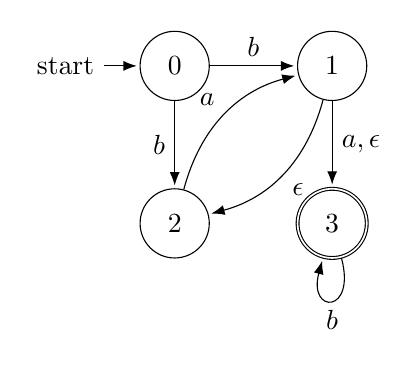
\begin{tikzpicture}[
    node distance=2cm, 
    on grid, 
    auto,
    >=Latex,
    shorten >=1pt
]
    \node[state, initial] (q0) {0};
    \node[state] (q1) [right=of q0] {1};
    \node[state] (q2) [below=of q0] {2};
    \node[state, accepting] (q3) [below=of q1] {3};

    \path[->]
        (q0) edge node {$b$} (q1)
        (q0) edge node[swap] {$b$} (q2)
        (q1) edge[bend left] node {$\epsilon$} (q2)
        (q1) edge node {$a, \epsilon$} (q3)
        (q2) edge[bend left] node {$a$} (q1)
        (q3) edge[loop below] node {$b$} ();
\end{tikzpicture}
\end{center}

\end{document}